\fuxiti
\begin{xiaotis}
\begin{enhancedline}

\xiaoti{已知: $O$ 是 $\triangle ABC$ 内的一点。求证:}
\begin{xiaoxiaotis}

    \xxt{$\angle BOC > \angle A$;}

    \xxt{$\exdfrac{1}{2} (BC + CA + AB) < OA + OB + OC$。}

\end{xiaoxiaotis}


\xiaoti{已知: $\triangle ABC$ 的 $\angle B$ 和 $\angle C$ 的平分线 $BE$、$CF$ 交于点 $I$。求证:}
\begin{xiaoxiaotis}

    \xxt{$\angle BIC = 180^\circ - \exdfrac{1}{2} (\angle ABC + \angle ACB)$;}

    \xxt{$\angle BIC = 90^\circ + \exdfrac{1}{2} \angle A$。}

\end{xiaoxiaotis}


\xiaoti{有星形如图,求证: $\angle A + \angle B + \angle C + \angle D + \angle E = 180^\circ$。}

\begin{figure}[htbp]
    \centering
    \begin{minipage}[b]{7cm}
        \centering
        \begin{tikzpicture}
    \tkzDefPoints{0/0/C, 2/0/D}
    \tkzDefRegPolygon[side,sides=5,name=P](C,D)

    % 为了绘制的代码更简洁明了,先将 P5 这样的点重新命名
    % \coordinate 是 tikz 的语句,而非 tkz-euclide 的。
    % 如果不重命名,应该这样写:
    %    \tkzDrawSegments(P4,C  C,P3  P3,P5  P5,D  D,P4)
    %    \tkzLabelPoints[above](P4){$A$}
    %    ...
    \coordinate (A) at (P4);
    \coordinate (B) at (P5);
    \coordinate (E) at (P3);

    \tkzDrawSegments(A,C  C,E  E,B  B,D  D,A)
    \tkzLabelPoints[above](A)
    \tkzLabelPoints[left](B,C)
    \tkzLabelPoints[right](D,E)
\end{tikzpicture}


        \caption*{(第 3 题)}
    \end{minipage}
    \qquad
    \begin{minipage}[b]{7cm}
        \centering
        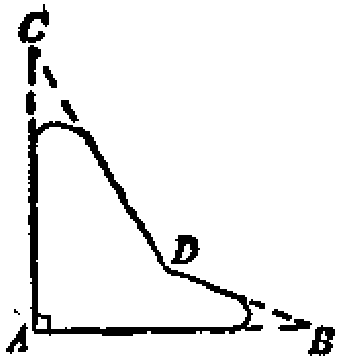
\includegraphics[width=3.8cm]{../pic/czjh1-ch3-fuxi-04.png}
        \caption*{(第 4 题)}
    \end{minipage}
\end{figure}

\xiaoti{一个零件的形状如图,按规定 $\angle A$ 应等于 $90^\circ$, $\angle B$、 $\angle C$
    应分别是 $21^\circ$ 和 $32^\circ$。 检验工人量得 $\angle BDC = 148^\circ$,
    就断定这个零件不合格,这是为什么呢?
}


\xiaoti{求证: 如果延长 $\triangle ABC$ 的中线 $AD$ 至 $A'$, 使 $DA' = AD$, 那么 $A'C = AB$。}

\xiaoti{求证: 全等三角形对应边上的中线相等。}

\xiaoti{求证: 三角形一条边的两端到这边上的中线或中线延长线的距离相等。}

\xiaoti{求证: 如果两个三角形有两个角和第三个角的角平分线对应相等,那么这两个三角形全等。}


\xiaoti{}%
\begin{xiaoxiaotis}%
    \xxt[\xxtsep]{在 $\angle AOB$ 的 $OA$ 边上取两点 $P$ 和 $S$, 再在 $OB$ 边上取两点 $Q$ 和 $T$,
        使 $OQ = OP$, $OT = OS$, $PT$ 和 $QS$ 相交于点 $X$。\\
        求证: $OX$  平分 $\angle AOB$;
    }

    \xxt{根据(1) 设计一种作已知角的平分线的方法。}

\end{xiaoxiaotis}


\xiaoti{已知:如图, 点 $C$ 为线段 $AB$ 上一点, $\triangle ACM$、 $\triangle CBN$ 是等边三角形。\\
    求证: $AN = BM$。
}

\begin{figure}[htbp]
    \centering
    \begin{minipage}[b]{4.6cm}
        \centering
        \begin{tikzpicture}
    \tkzDefPoints{0/0/A, 4/0/B, 1.5/0/C}
    \tkzDefTriangle[equilateral](A,C)  \tkzGetPoint{M}
    \tkzDefTriangle[equilateral](C,B)  \tkzGetPoint{N}

    \tkzDrawPolygon(A,C,M)
    \tkzDrawPolygon(B,C,N)
    \tkzDrawSegments(A,N  B,M)
    \tkzLabelPoints[above](M,N)
    \tkzLabelPoints[below](A,B,C)
\end{tikzpicture}


        \caption*{(第 10 题)}
    \end{minipage}
    \qquad
    \begin{minipage}[b]{4.6cm}
        \centering
        \begin{tikzpicture}
    \tkzDefPoints{0/0/B, 4/0/C}
    \tkzDefTriangle[equilateral](B,C)  \tkzGetPoint{A}
    \tkzDefPointOnLine[pos=0.7](A,B)  \tkzGetPoint{D}
    \tkzDefPointOnLine[pos=0.7](B,C)  \tkzGetPoint{E}
    \tkzDefPointOnLine[pos=0.7](C,A)  \tkzGetPoint{F}

    \tkzDrawPolygon(A,B,C)
    \tkzDrawPolygon(D,E,F)
    \tkzLabelPoints[above](A)
    \tkzLabelPoints[below](B,C,E)
    \tkzLabelPoints[left](D)
    \tkzLabelPoints[right, yshift=.3em](F)
\end{tikzpicture}


        \caption*{(第 11 题)}
    \end{minipage}
    \qquad
    \begin{minipage}[b]{4.5cm}
        \centering
        \begin{tikzpicture}
    \pgfmathsetmacro{\r}{1.3}
    \tkzDefPoints{0/0/B, \r/0/P, 2*\r/0/Q, 3*\r/0/C}
    \tkzInterCC[R](P,\r)(Q,\r)  \tkzGetFirstPoint{A}

    \tkzDrawSegments(A,B  A,C  A,P  A,Q  B,C)
    \tkzLabelPoints[above](A)
    \tkzLabelPoints[below](B,C,P,Q)
\end{tikzpicture}


        \caption*{(第 13 题)}
    \end{minipage}
\end{figure}

\xiaoti{在等边三角形 $ABC$ 的三边上,分别取点 $D$、$E$、$F$, 使 $AD = BE = CF$。 \\
    求证: $\triangle DEF$ 是等边三角形。
}

\xiaoti{已知; $\triangle ABC$ 中, $I$ 是角平分线 $BE$ 和 $CF$ 的交点,
    $MN$ 经过 $I$, 平行于 $BC$, 交 $AB$ 于点 $M$, 交 $AC$ 于点 $N$。 \\
    求证: $MN = BM + CN$。
}

\xiaoti{已知 $P$、 $Q$ 是 $\triangle ABC$ 的边 $BC$ 上两点,
    并且 $BP = PQ = QC = AP = AQ$, 求 $\angle BAC$ 的大小。
}

\xiaoti{求证: 如果把等腰三角形的底边向两方向分别延长相等线段,那么延长线段的两个外端与等腰三角形的顶点距离相等。}

\xiaoti{已知: $AB$ 是等腰直角三角形 $ABC$ 的斜边, $AD$ 是 $\angle A$ 的平分线。 求证:$AC + CD = AB$。}

\xiaoti{已知: $\triangle ABC$ 中, $AB = AC$, $E$ 是 $AB$ 上一点, $F$ 是 $AC$ 延长线上一点,
    $BE = CF$, $EF$ 交 $BC$ 于 $D$。 求证: $DE = DF$。
}

\xiaoti{已知: $DC \pingxing AB$, $O$ 是 $AC$ 和 $BD$ 的交点, $OA < OB$。求证: $OC < OD$。}

\begin{figure}[htbp]
    \centering
    \begin{minipage}[b]{4.6cm}
        \centering
        \begin{tikzpicture}
    \tkzDefPoints{0/0/A, 4/0/B, 0.5/2.5/D,  2.5/2.5/C}
    \tkzInterLL(A,C)(B,D)  \tkzGetPoint{O}

    \tkzDrawPolygon(A,B,D,C)
    \tkzLabelPoints[above](C,D)
    \tkzLabelPoints[below](A,B)
    \tkzLabelPoints[left,xshift=-.3em](O)

    % OA < OB
    % \tkzCalcLength(O,A)  \tkzLabelSegment(O,A){$\tkzLengthResult$}
    % \tkzCalcLength(O,B)  \tkzLabelSegment(O,B){$\tkzLengthResult$}
\end{tikzpicture}


        \caption*{(第 17 题)}
    \end{minipage}
    \qquad
    \begin{minipage}[b]{4.6cm}
        \centering
        \begin{tikzpicture}
    \tkzDefPoints{0/0/B, 4/0/C, 1/2/A}
    \tkzDefMidPoint(B,C)  \tkzGetPoint{D}

    \tkzDrawPolygon(A,B,C)
    \tkzDrawSegment(A,D)
    \tkzLabelPoints[above](A)
    \tkzLabelPoints[below](B,C,D)

    % 角 BAD > 角 DAC
    % \tkzFindAngle(B,A,D) \tkzGetAngle{an} \tkzLabelAngle(B,A,D){$\pgfmathprintnumber{\an}$}
    % \tkzFindAngle(D,A,C) \tkzGetAngle{an} \tkzLabelAngle[pos=0.5](D,A,C){$\pgfmathprintnumber{\an}$}
\end{tikzpicture}


        \caption*{(第 18 题)}
    \end{minipage}
    \qquad
    \begin{minipage}[b]{4.5cm}
        \centering
        \begin{tikzpicture}
    \tkzDefPoints{0/0/B, 3/0/C}
    \tkzDefTriangle[two angles=60 and 75](B,C)  \tkzGetPoint{A}
    \tkzDefLine[altitude](B,A,C)  \tkzGetPoint{D}
    \tkzDefLine[altitude](A,B,C)  \tkzGetPoint{E}
    \tkzInterLL(A,D)(B,E)  \tkzGetPoint{H}

    \tkzDrawPolygon(A,B,C)
    \tkzDrawSegments(A,D  B,E)
    \tkzMarkRightAngle(A,D,B)
    \tkzMarkRightAngle(B,E,C)
    \tkzLabelPoints[above](A)
    \tkzLabelPoints[below](B,C,D)
    \tkzLabelPoints[right](E)
    \tkzLabelPoints[above left](H)
\end{tikzpicture}


        \caption*{(第 19 题)}
    \end{minipage}
\end{figure}

\xiaoti{已知: $AD$ 是 $\triangle ABC$ 的中线, $\angle BAD > \angle DAC$。 求证: $AC > AB$。\\
    (提示: 延长 $AD$ 到 $A'$, 使 $DA' = AD$, 连续 $BA'$, 先证明 $\triangle ADC \quandeng \triangle A'DB$。)
}

\xiaoti{已知:$\triangle ABC$ 中, $\angle ABC = 45^\circ$, $H$ 是高 $AD$ 和 $BE$ 的交点。 求证:$BH = AC$。}

\xiaoti{求证: 等腰三角形腰上的高与底边的夹角等于顶角的一半。}

\xiaoti{已知: $\triangle ABC$ 中 $BE$、$CF$ 是高,$M$ 是 $BC$ 的中点, $N$ 是 $EF$ 的中点。\\
    求证: (1)$ME = MF$; (2) $MN \perp EF$。
}

\xiaoti{已知: $\triangle ABC$ 中, $AD$ 是 $BC$ 上的高, $AB = AC = 2 AD$,
    $DE \perp AB$, $DF \perp AC$, 垂足分别是 $E$、 $F$。 \\
    求证: $DE + DF = \exdfrac{1}{2} BC$。
}

\xiaoti{求证: 两个锐角三角形有两边和其中一边上的高对应相等,那么这两个三角形全等。}

\xiaoti{求作等腰直角三角形, 使它的斜边等于已知线段。}

\xiaoti{写出下列定理的逆命题, 并且说明它们是不是真命题:}
\begin{xiaoxiaotis}

    \xxt{如果 $a = 2$, 那么 $a^2 = 4$;}

    \xxt{如果一个整数的个位数字是 $5$, 那么这个数能被 $5$ 整除;}

    \xxt{如果两个三角形全等, 那么它们的对应角相等。}

\end{xiaoxiaotis}


\xiaoti{已知: $\triangle ABC$ 中, $AB = AC$, $AD$ 是 $BC$ 边上的中线,
    $AB$ 的垂直平分线交 $AD$ 于点 $O$, $\angle B$ 的平分线交 $AD$ 于点 $I$。\\
    求证:(1) $OA = OB = OC$; \\
    (2) $I$ 到 $BC$、$CA$、$AB$ 的距离相等。
}

\xiaoti{下列图形, 如果有对称轴, 作出它们的对称轴:}

\begin{figure}[htbp]
    \centering
    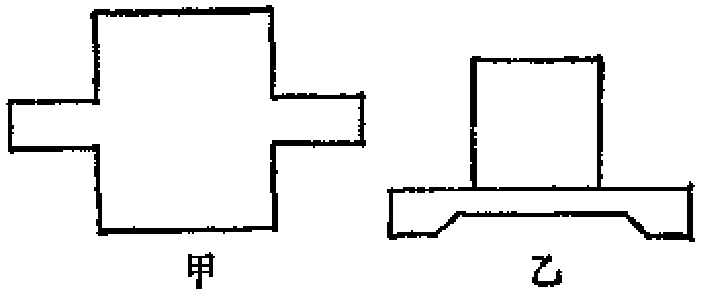
\includegraphics[width=9cm]{../pic/czjh1-ch3-fuxi-27.png}
    \caption*{(第 27 题)}
\end{figure}

\end{enhancedline}
\end{xiaotis}

